\documentclass[UTF8,hyperref]{article}
\usepackage[utf8]{inputenc}
\usepackage{hyperref}
\usepackage{amsmath}
\usepackage{amsfonts}
\usepackage{amssymb}
\usepackage{amsthm}
\usepackage{graphicx}
\usepackage{caption}
\usepackage{subfigure}
\usepackage{listings}
\usepackage{xcolor}

\title{Numerical Analysis Project}
\author{Rui Sun}
\date{December 2021}

\begin{document}

\maketitle

\section{Lagrange Polynomial}

\subsection{Problem (a)}
\par Let $f(x)=\dfrac{1}{1+25x^2}$ be a function in $[-1,1]$, and let $p_n(x)$ be the polynomial of degree at most $n$ that interpolates the function $f$ at $n+1$ equally-spaced points $x_0,x_1,\cdots,x_n$ in the interval $[-1,1]$. Thus one gets
\begin{equation}
    h=\frac{2.0}{n}, x_k=-1.0+kh, k=0,1,\cdots,n
\end{equation}
.
\par $p_n(x)$ is an approximation of $f(x)$ at these points. Choose $n=5,10,20$ and compute $p_n(x)$ at
$$
x=-0.95,-0.47,0.1,0.37,0.93
$$
and compare them with $f(x)$ at these points.

\paragraph{Solution} A Python program was created to solve for the value of the polynomial obtained by Lagrangian interpolation at a given point, and a plot of the interpolated polynomial against the original function was drawn.
The following outputs are the errors:

\lstset{
 columns=fixed,       
 numbers=none,
 numberstyle=\tiny\color{gray},
 keywordstyle=\color[RGB]{230,125,85},
 numberstyle=\footnotesize\color{darkgray},           
 commentstyle=\it\color[RGB]{80,175,96},
 stringstyle=\rmfamily\slshape\color[RGB]{128,0,0},
 showstringspaces=false,
 basicstyle=\ttfamily,
}
\begin{lstlisting}
n = 5:
f(-0.95)-p_n(-0.95) = 0.05817799859084909
f(-0.47)-p_n(-0.47) = -0.09031533471876207
f(0.1)-p_n(0.1) = 0.2498798076923081
f(0.37)-p_n(0.37) = -0.12677490820134119
f(0.93)-p_n(0.93) = 0.07473742125006333

n = 10:
f(-0.95)-p_n(-0.95) = -1.8811908314168162
f(-0.47)-p_n(-0.47) = -0.0936037537592041
f(0.1)-p_n(0.1) = -0.04340742982890311
f(0.37)-p_n(0.37) = 0.03707696272967939
f(0.93)-p_n(0.93) = -1.8837448249769186

n = 20:
f(-0.95)-p_n(-0.95) = 39.99488935134396
f(-0.47)-p_n(-0.47) = -0.014037800024217284
f(0.1)-p_n(0.1) = -6.661338147750939e-16
f(0.37)-p_n(0.37) = 0.006985095986455858
f(0.93)-p_n(0.93) = 18.598125682561882
\end{lstlisting}
\par The plots generated are listed here:
\begin{figure}[htbp]
    \centering
    \subfigure[$n=5$]{
        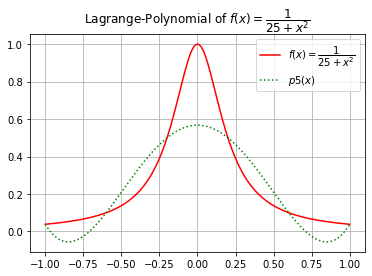
\includegraphics[scale=0.5]{img_results/pic1.png}
        \label{Fig1.a}
    }
    \quad
    \subfigure[$n=10$]{
        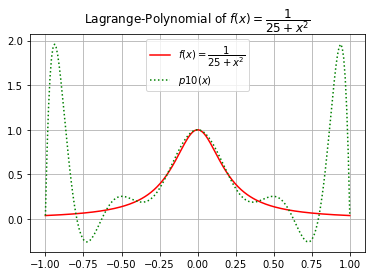
\includegraphics[scale=0.5]{img_results/pic2.png}
        \label{Fig1.b}
    }
    \quad
    \subfigure[$n=20$]{
        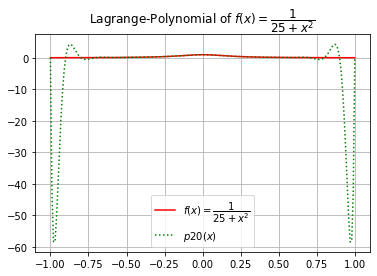
\includegraphics[scale=0.5]{img_results/pic3.png}
        \label{Fig1.c}
    }
    \caption{Comparison of function $f(x)=\dfrac{1}{1+25x^2}$ and interpolated polynomial}
    \label{Fig1}
\end{figure}
\par From the errors outputed and Figure \ref{Fig1}, it's clear that the value of the interpolating polynomial deviates significantly from the value of the original function near the boundaries of the range. And with the increase of $n$, the errors also increase. This is called Runge phenomenon.

\subsection{Problem (b)}
\par Let $f(x)=e^x$ be a function in $[-1,1]$ and $p_n(x)$ be the interpolating polynomia of $n+1$ equally-spaced points. Choose $n=5,10,20$ and compute $p_n(x)$ at $x=-0.95,-0.47, 0.1,0.37,0.93$ and compare them with $f(x)$ at these points.

\par Discribe your observation. Based on your observation, do you think the higher the interpolating polynomial degree, the better?
\paragraph{Solution} With the same method, the errors are calculated and displayed as follow (To make things clear, we replace $f(x)=e^x$ with $g(x)=e^x$):

\begin{lstlisting}
n = 5:
g(-0.95)-p_n(-0.95) = -5.713540349228108e-05
g(-0.47)-p_n(-0.47) = 2.6157349590438805e-05
g(0.1)-p_n(0.1) = -1.5015848680688393e-05
g(0.37)-p_n(0.37) = 2.8034715736424687e-05
g(0.93)-p_n(0.93) = -9.20797823367181e-05

n = 10:
g(-0.95)-p_n(-0.95) = 1.9882628876644048e-10
g(-0.47)-p_n(-0.47) = 5.749622999928761e-12
g(0.1)-p_n(0.1) = -2.517097641430155e-12
g(0.37)-p_n(0.37) = 2.1027624086400465e-12
g(0.93)-p_n(0.93) = -2.283302436012491e-10

n = 20:
g(-0.95)-p_n(-0.95) = -6.306066779870889e-14
g(-0.47)-p_n(-0.47) = 1.1102230246251565e-16
g(0.1)-p_n(0.1) = -8.881784197001252e-16
g(0.37)-p_n(0.37) = 0.0
g(0.93)-p_n(0.93) = 4.929390229335695e-14
\end{lstlisting}
\begin{figure}[htbp]
    \centering
    \subfigure[$n=5$]{
        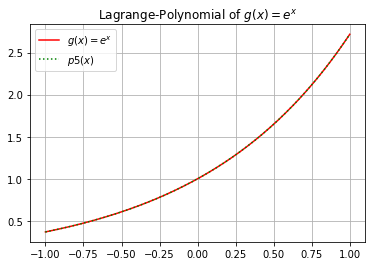
\includegraphics[scale=0.5]{img_results/pic4.png}
        \label{Fig2.a}
    }
    \quad
    \subfigure[$n=10$]{
        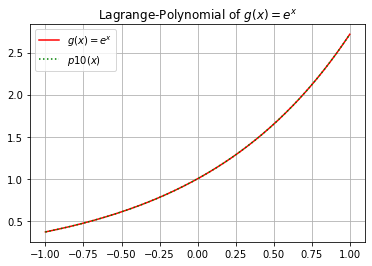
\includegraphics[scale=0.5]{img_results/pic5.png}
        \label{Fig2.b}
    }
    \quad
    \subfigure[$n=20$]{
        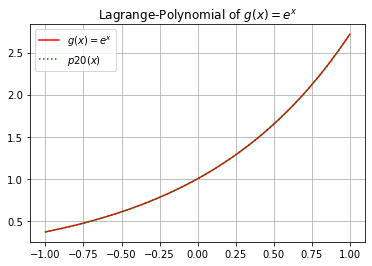
\includegraphics[scale=0.5]{img_results/pic6.png}
        \label{Fig2.c}
    }
    \caption{Comparison of function $g(x)=e^x$ and interpolated polynomial}
    \label{Fig2}
\end{figure}
\par Things are completely different with $g(x)=e^x$. The errors were extremely small, and with the increase of $n$, the errors go down. From Figure \ref{Fig2}, it shows clearly that even for a small $n$, the interpolated polynomial fits the original function perfectly.
\par For diffetent functions, it's not the larger $n$, the more perfect the interpolated polynomial.

\subsection{Problem (c)}

\par Let $f(x)=\dfrac{1}{25+x^2}$ be a function in $[-1,1]$ and consider the interpolating polynomial with respect to thr distinct points $x_i=\cos{\dfrac{(2k+1)\pi}{2(n+1)}},\, k=0,1,\cdots,n$. Choose $n=5,10,20$ and compare them with $f(x)$ at these points.

\par Describe the observation. Read reference [1], p.315-323 and explain this phenomenon.

\paragraph{Solution} Use the improved method, the results are outputed.
\begin{lstlisting}
n = 5:
f(-0.95)-p_n(-0.95) = 0.007747003469783263
f(-0.47)-p_n(-0.47) = -0.08343042460406644
f(0.1)-p_n(0.1) = 0.3667983064716973
f(0.37)-p_n(0.37) = -0.08129139149124548
f(0.93)-p_n(0.93) = 0.015594529058462814

n = 10:
f(-0.95)-p_n(-0.95) = -0.043094613035724004
f(-0.47)-p_n(-0.47) = 0.06431306024108874
f(0.1)-p_n(0.1) = -0.08124703825599944
f(0.37)-p_n(0.37) = 0.08153549403081947
f(0.93)-p_n(0.93) = -0.025341946966374165

n = 20:
f(-0.95)-p_n(-0.95) = -0.0057596689619212466
f(-0.47)-p_n(-0.47) = 0.00834879653818646
f(0.1)-p_n(0.1) = -0.010624838022320393
f(0.37)-p_n(0.37) = -0.012827402039512492
f(0.93)-p_n(0.93) = 0.00031722267527464765
\end{lstlisting}
\begin{figure}[htbp]
    \centering
    \subfigure[$n=5$]{
        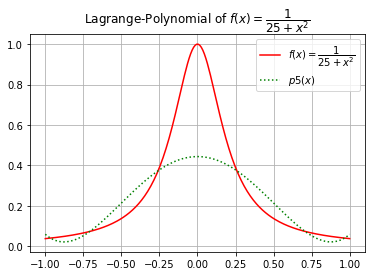
\includegraphics[scale=0.5]{img_results/pic7.png}
        \label{Fig3.a}
    }
    \quad
    \subfigure[$n=10$]{
        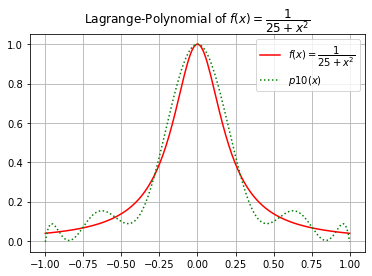
\includegraphics[scale=0.5]{img_results/pic8.png}
        \label{Fig3.b}
    }
    \quad
    \subfigure[$n=20$]{
        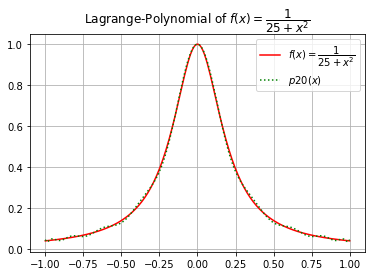
\includegraphics[scale=0.5]{img_results/pic9.png}
        \label{Fig3.c}
    }
    \caption{Comparison of function $f(x)=\dfrac{1}{1+25x^2}$ and interpolated polynomial}
    \label{Fig3}
\end{figure}

\par According to Figure \ref{Fig3}, when replace equidistant nodes with Chebyshev nodes, the errors converge to $0$ with the increase of $n$. Whether or not the Runge phenomenon appears is related to the selection of the interpolation node set.

\par In Probelm (a), the Runge phenomenon appears because of 
\begin{equation}
\lim_{n\rightarrow \infty}{(\max_{-1\le x \le 1}{\vert f(x)-P_n(x)\vert })}=\infty
\end{equation}
. 
\par The errors of interpolated polynomial comes from higher order remainder term of Taylor expansion.
\begin{equation}
    f(x)-P_n(x)=\dfrac{f^{(n+1)}(\xi)}{(n+1)!}\prod_{i=0}^{n}(x-x_i)
\end{equation}.
\par For some $\xi$ in range $(-1,1)$, there is:
\begin{equation}
    \max_{-1\le x \le 1}{|f(x)-P_n(x)|}\le \max_{-1\le x \le 1}{\dfrac{|f^{(n+1)}(x)|}{(n+1)!}}\max_{-1 \le x\le 1}{\prod_{i=0}^{n}{|x-x_i|}}
\end{equation}.
\par Define $w(x)$ to be the nodal function:
\begin{equation}
    w_n(x)=\prod_{i=1}^{n}{(x-x_i)}
\end{equation}
.
\par It's hard to solve $\displaystyle \max_{-1\le x \le 1}{|f^{(n+1)}(x)|}$, consider Cauchy's integral formula:
\begin{equation}
    f^{(n)}(\xi)=\dfrac{n!}{2\pi j}{\int_C{\dfrac{f(z)}{(z-\xi)^{n+1}}}\mathrm{d}z}
\end{equation}, now we can solve the errors:
\begin{equation}
    f(z)-P_n(z)=\dfrac{1}{2\pi j}{\int_C{\dfrac{w_n(z)f(\xi)}{w_n(\xi)(\xi-z)}}\mathrm{d}\xi}
\end{equation}
,$C$ is the boundary of domain $D$. According to the conditions of Cauchy's integral formula, $f$ is a holomorphic function in $D$, and all the interpolation nodes should be in $D$.
\par For a sufficiently large $r$, $w_n(z)=r^n$ is nearly a circle. Use $C^*:w_n(\xi)=r^n$ as the loop of integration. For all $z$ in $C^*$,$\displaystyle \lim_{n\rightarrow\infty}{|\dfrac{w_n(z)}{w_n(\xi)}|}=0$. For all $z$ out of $C^*$, $\displaystyle \lim_{n\rightarrow\infty}{|\dfrac{w_n(z)}{w_n(\xi)}|}=\infty$. When the singularities of $f(z)$:$z_1=\dfrac{j}{5},\,z_2=-\dfrac{j}{5}$ are in $C^*$, $f(z)-P_n(z)$ goes towards to infinity.
\par When we replace equidistant nodes with Chebyshev nodes, $w_n(z)=r^n$ becomes a ellipse with focuses $\pm 1$. Singularities $\pm \dfrac{j}{5}$ are out of $C^*$, so $f(z)-P_n(z)$ goes towards to zero. The Runge phenomenon disappeared.

\section{Numerical Integration}
\subsection{Problem (a)}
\par To compute the integral $\displaystyle\int_{a}^{b}{f(x)}\mathrm{d}x$ numerically, one can use the Romberg integration formula. To be more specific, let $R(n, 0)$ denote the trapezoid estimate with $2^n$ subintervals, we have the Romberg formula:

\begin{equation}
\begin{cases}
R(0,0)=\dfrac{1}{2}(b-a)[f(a)+f(b)],\\
\displaystyle{R(n,0)=\dfrac{1}{2}R(n-1,0)+h_n\sum_{i=1}^{2^{n-1}}{f(a+(2i-1)h_n)}}
\end{cases}
\end{equation}
where 
\begin{equation}
h_0=b-a, h_n=\dfrac{h_{n-1}}{2}
\end{equation}.
\par Use Romberg integration to compute the following integrals with the tolerance of accuracy to be $\epsilon=10^{-7}$, which means if $[R(n+1,0)-R(n,0)]\le\epsilon$, then we use $R(n,0)$ as the desired numerical integration.

\begin{itemize}
    \item (a) $\displaystyle{\int_{0}^{1}{x^2e^x}\mathrm{d}x}$
    \item (b) $\displaystyle{\int_{1}^{3}{e^x\sin{x}}\mathrm{d}x}$
    \item (c) $\displaystyle{\int_{0}^{1}{\dfrac{4}{1+x^2}}\mathrm{d}x}$
    \item (d) $\displaystyle{\int_{0}^{1}{\dfrac{1}{x+1}}\mathrm{d}x}$
\end{itemize}

\paragraph{Solution} First, solve for the parsing solutions:
\begin{equation}
    \begin{aligned}
        \displaystyle{\int_{0}^{1}{x^2e^x}\mathrm{d}x} =e-2\\
        \displaystyle{\int_{1}^{3}{e^x\sin{x}}\mathrm{d}x}=\frac{e}{2}(-\sin{1}+\cos{1}+e^2(\sin{3}-\cos{3})) \\
        \displaystyle{\int_{0}^{1}{\dfrac{4}{1+x^2}}\mathrm{d}x}=\pi \\
        \displaystyle{\int_{0}^{1}{\dfrac{1}{x+1}}\mathrm{d}x}=\ln{2}
    \end{aligned}
\end{equation}
The Romberg integration algorithm is simple. There comes the results:
\begin{lstlisting}
Romberg Integration

f(x) = x^2 e^x
a = 0, b = 1
I =  0.7182818385854369

f(x) = e^x sin(x)
a = 1, b = 3
I =  10.950170288849279

f(x) = 4/(1+x^2)
a = 0, b = 1
I =  3.1415926436556827

f(x) = 1/(1+x)
a = 0, b = 1
I =  0.6931471954611083
\end{lstlisting}
\par Errors are less than $\epsilon$.

\subsection{Problem (b)}
\par Use Gauss-Legendre quadrature rule to compute the above integrals to $\epsilon=10^{-7}$ and compare the number of quadrature points used.
\paragraph{Solution} The code to generate the weights and Gauss nodes are not given. So it's necessary to write it by myself. There comes the results:
\begin{lstlisting}
Gauss-Legendre Integration

f(x) = x^2 e^x
a = 0, b = 1
I =  0.718281828393355

f(x) = e^x sin(x)
a = 1, b = 3
I =  10.95017031533695

f(x) = 4/(1+x^2)
a = 0, b = 1
I =  3.1415926111875865

f(x) = 1/(1+x)
a = 0, b = 1
I =  0.6931471798865281
\end{lstlisting}
\par Errors are less than $\epsilon$.

\subsection{Problem (c)}
\par Compute $\displaystyle{\int_{-\infty}^{+\infty}}{e^{-x^2}\mathrm{d}x}$ to the tolerance of accuracy $\epsilon =10^{-7}$. ( Hint: although the integral is in unbounded domain, the integrand itself decays fast. )
\paragraph{Solution} The parsing solution:
\begin{equation}
    \int_{-\infty}^{+\infty}{e^{-x^2}}\mathrm{d}x=\sqrt{\pi}
\end{equation}
\begin{figure}[htbp]
    \centering
    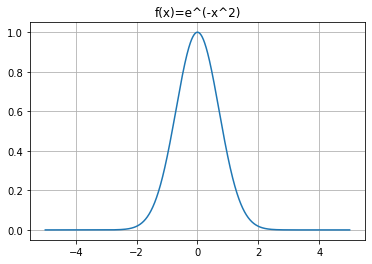
\includegraphics[scale=0.5]{img_results/pic10.png}
    \caption{Function $f(x)=e^{-x^2}$}
    \label{Fig4}
\end{figure}
\par The function's plot is Figure \ref{Fig4}. When $|x|$ increases, $f(x)$ converge to 0 rapidly. Calculate the integration from $-5$ to $5$ using two methods:
\begin{lstlisting}
Romberg Integration
I = 1.7724538509008183

Gauss-Legendre Integration
I = 1.772453844220363
\end{lstlisting}
\par Errors are less than $\epsilon$.
\end{document}